\documentclass[11pt]{article}
\usepackage[top=30truemm,bottom=30truemm,left=25truemm,right=25truemm]{geometry}
\usepackage[dvipdfmx]{graphicx}
\usepackage{float}
\begin{document}
\title{伝搬光-SPPカップラー}
\author{平松}
\maketitle

\abstract
伝搬光-SPPカップラーの設計について、先行研究や我々のシミュレーション、実験によって知られている知見をまとめる。

\section{溝深さ}
溝深さは1$\mu m$程度が最適である。\\
SPP励起効率は溝深さに強く依存する。適切なSPP溝深さでなければ、SPP励起効率は簡単に1/10以下になる\cite{pitch_grating}。\\
RCWAによるシミュレーションでは、図に示すように中赤外域において0.5$\mu m$から0.8$\mu m$程度の溝深さが最適だと予想される。ただしこの結果はグレーティングの長さが無限大だとする近似の上で導かれた結論であって、有限の長さをもつグレーティングにはこれ以上の溝深さが最適であると言える。\\
\begin{figure}[H]
\centering
  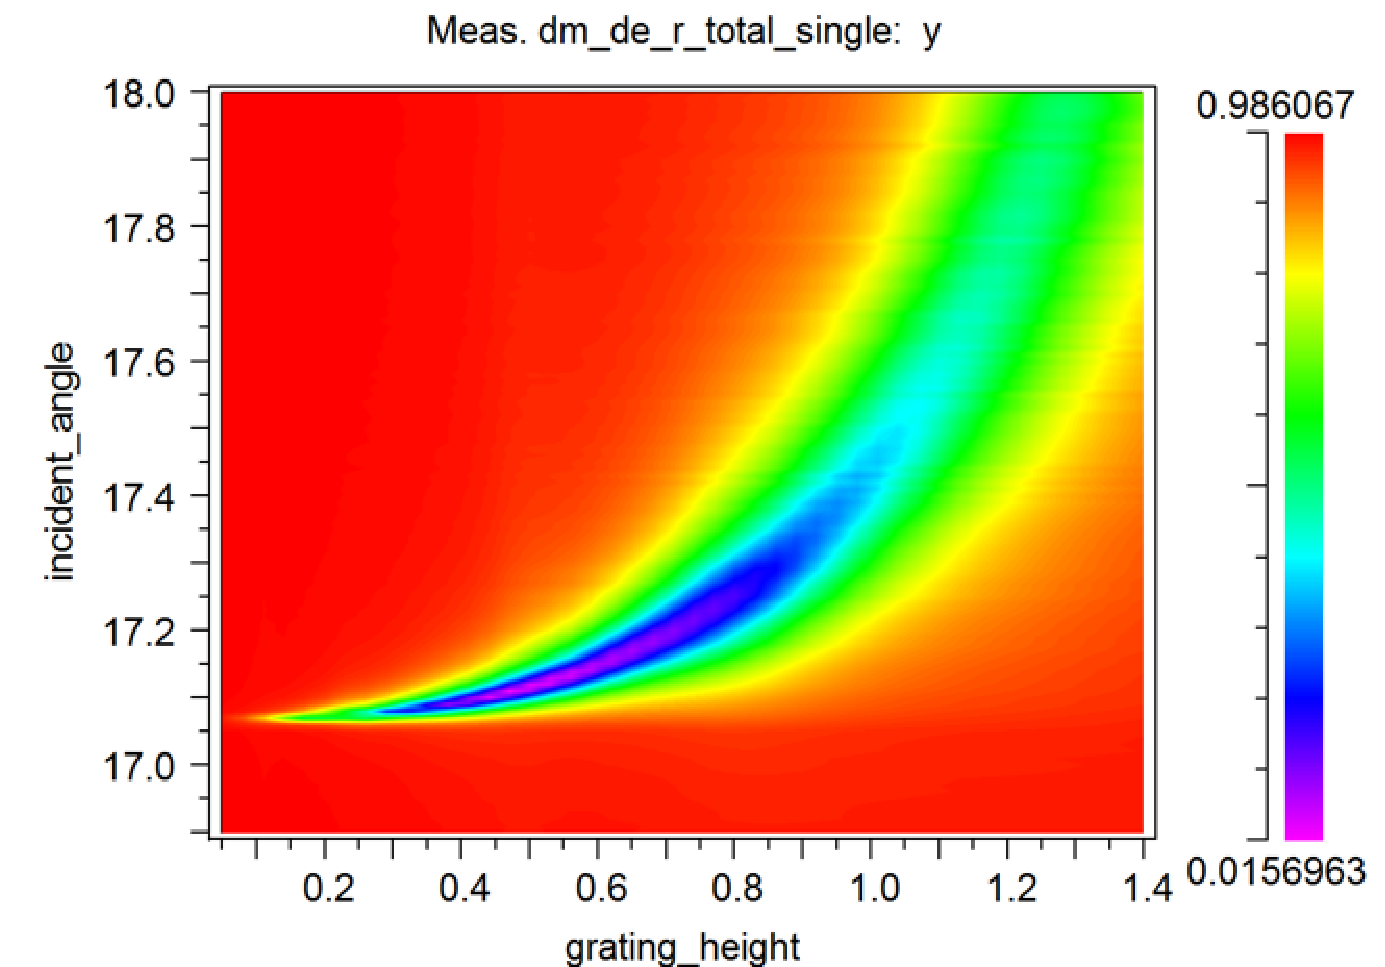
\includegraphics[width=10cm]{./RCWA.pdf}
\end{figure}
これは中赤外域において、溝深さが波長の10$\%$から15$\%$程度必要と主張する先行論文と矛盾しない\cite{Anneal_MIR_grating}。

\section{溝周期}
SPPを効率良く励起するための溝周期について以下の関係が導かれている\cite{pitch_grating}。
\begin{equation}k_{SPP}/k_0 < \lambda / d < k_{SPP}/k_0 +1\end{equation}
ただしdは溝の周期、$\lambda$は励起光の波長、$k_{SPP}$はSPPの波数、$k_0$は伝搬光の波数である。\\金を赤外域で伝搬するSPPの波数は伝搬光の波数に非常に近いので、近似的に、\\
\begin{equation}1 < \lambda / d < 2\end{equation}

\subsection{導出}
\begin{itemize}
\item SPPと伝搬光の波数整合条件$k_{SPP}=k_0 sin \theta + 2n \pi /d$ から$\lambda /d < k_{spp}/k_0 +1$が導かれる。ただし$\theta$は励起光の入射角。
\item incouple光の垂直入射は避けるべき\\
- 対称性よりSPPのエネルギーを2つに分けるため
\item 反射光(0次の回折光)以外の回折光が出ないような条件にすべき\\
- 回折光によるパワーロスを防ぐため\\
- 回折光に関する条件$k_0(sin \theta_m - sin \theta_i ) = 2 \pi m / d$を満たさないことから、
$k_{SPP}/k_0 < \lambda / d$が導かれる
\end{itemize}

\bibliographystyle{unsrt}
\bibliography{../Reference}

\end{document}
